\trilingualchapter{Location and Design: Creating the Perfect Space}{选址与设计:创造完美空间}{Standort und Design: Den perfekten Raum schaffen}{}

The location of a restaurant can make or break its success. Similarly, the design and ambiance play crucial roles in creating the dining experience. This chapter follows Sue and Owen as they search for the perfect location and design a space that reflects their concept.

\section{The Search for the Perfect Location | 寻找完美位置 | Die Suche nach dem perfekten Standort}

Sue and Owen spent three months searching for the ideal location. They knew that location was one of the most critical decisions they would make, affecting everything from foot traffic to operating costs.

\subsection{Location Criteria}

They established clear criteria for their location search:

\subsubsection{Visibility and Accessibility}
\begin{itemize}
    \item High visibility from main streets
    \item Easy access for pedestrians and vehicles
    \item Adequate parking (at least 1 space per 3 seats)
    \item Public transportation proximity
    \item Safe, well-lit area
\end{itemize}

\subsubsection{Demographics and Foot Traffic}
\begin{itemize}
    \item Target demographic presence
    \item Daytime and evening foot traffic
    \item Nearby businesses that complement the restaurant
    \item Residential density
    \item Tourist traffic (if applicable)
\end{itemize}

\subsubsection{Physical Requirements}
\begin{itemize}
    \item Minimum 2,500 square feet
    \item Adequate ceiling height (at least 10 feet)
    \item Proper ventilation and exhaust systems
    \item Sufficient electrical capacity (minimum 400 amps)
    \item Gas line availability
    \item Water and sewer capacity
    \item Loading dock or delivery access
\end{itemize}

\subsubsection{Financial Considerations}
\begin{itemize}
    \item Rent within budget (typically 6-10\% of gross sales)
    \item Lease terms and flexibility
    \item Common area maintenance (CAM) fees
    \item Property taxes and insurance
    \item Utilities included or separate
    \item Tenant improvement allowance
\end{itemize}

\subsection{Location Evaluation Process | 选址评估流程 | Standortbewertungsprozess}

For each potential location, Sue and Owen created an evaluation matrix:

\begin{table}[h]
\centering
\begin{tabular}{lcc}
\toprule
\textbf{Criteria} & \textbf{Weight} & \textbf{Score (1-10)} \\
\midrule
Visibility & 15\% & \\
Accessibility & 15\% & \\
Foot traffic & 20\% & \\
Demographics match & 15\% & \\
Size and layout & 10\% & \\
Rent and terms & 15\% & \\
Competition & 10\% & \\
\midrule
\textbf{Total} & \textbf{100\%} & \\
\bottomrule
\end{tabular}
\caption{Location Evaluation Matrix}
\end{table}

\section{Lease Negotiation | 租赁谈判 | Mietverhandlung}

After identifying their preferred location, Sue and Owen entered lease negotiations. Key points they addressed:

\subsection{Lease Terms | 租赁条款 | Mietbedingungen}
\begin{itemize}
    \item Lease duration (initial term and renewal options)
    \item Rent amount and escalation clauses
    \item Security deposit and personal guarantees
    \item Tenant improvement allowance
    \item Exclusivity clauses (preventing similar restaurants nearby)
    \item Assignment and subletting rights
    \item Termination clauses
\end{itemize}

\subsection{Important Clauses | 重要条款 | Wichtige Klauseln}
\begin{itemize}
    \item \textbf{Use clause}: Defines permitted uses
    \item \textbf{Operating hours}: Any restrictions on hours
    \item \textbf{Signage rights}: Exterior and interior signage
    \item \textbf{Maintenance responsibilities}: Who maintains what
    \item \textbf{Insurance requirements}: Minimum coverage amounts
    \item \textbf{Compliance}: Health codes, ADA, building codes
\end{itemize}

\section{Design Philosophy | 设计理念 | Designphilosophie}

With the location secured, Sue and Owen turned to design. Their design philosophy centered on creating a warm, inviting space that reflected their artisan bistro concept while ensuring operational efficiency.

\subsection{Design Principles | 设计原则 | Designprinzipien}

\begin{enumerate}
    \item \textbf{Authenticity}: Materials and finishes that feel genuine
    \item \textbf{Comfort}: Seating and spacing that encourages lingering
    \item \textbf{Efficiency}: Layout that supports smooth operations
    \item \textbf{Flexibility}: Spaces that can adapt to different needs
    \item \textbf{Sustainability}: Environmentally conscious choices
\end{enumerate}

\section{Space Planning | 空间规划 | Raumplanung}

\begin{figure}[h]
\centering
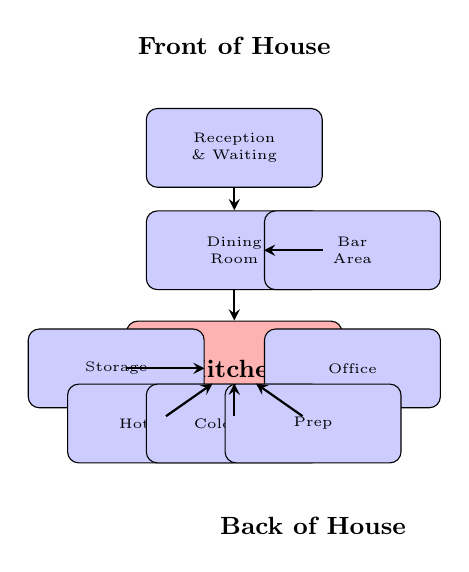
\begin{tikzpicture}[
    node distance=1cm,
    auto,
    room/.style={rectangle, draw, fill=blue!20, text width=2cm, text centered, rounded corners, minimum height=1cm, font=\tiny},
    kitchen/.style={rectangle, draw, fill=red!30, text width=2.5cm, text centered, rounded corners, minimum height=1.2cm, font=\small\bfseries},
    arrow/.style={thick,->,>=stealth}
]
    % Front of house
    \node [room] (dining) {Dining\\Room};
    \node [room, right of=dining, xshift=0.5cm] (bar) {Bar\\Area};
    \node [room, above of=dining, yshift=0.3cm] (reception) {Reception\\\& Waiting};
    
    % Back of house
    \node [kitchen, below of=dining, yshift=-0.5cm] (kitchen) {Kitchen};
    \node [room, left of=kitchen, xshift=-0.5cm] (storage) {Storage};
    \node [room, right of=kitchen, xshift=0.5cm] (office) {Office};
    
    % Kitchen stations
    \node [room, below of=kitchen, yshift=0.3cm, xshift=-1cm] (hot) {Hot Line};
    \node [room, below of=kitchen, yshift=0.3cm] (cold) {Cold Line};
    \node [room, below of=kitchen, yshift=0.3cm, xshift=1cm] (prep) {Prep};
    
    % Arrows
    \draw [arrow] (reception) -- (dining);
    \draw [arrow] (dining) -- (bar);
    \draw [arrow] (dining) -- (kitchen);
    \draw [arrow] (kitchen) -- (storage);
    \draw [arrow] (kitchen) -- (hot);
    \draw [arrow] (kitchen) -- (cold);
    \draw [arrow] (kitchen) -- (prep);
    
    % Labels
    \node [above of=reception, yshift=0.3cm, font=\small\bfseries] {Front of House};
    \node [below of=prep, yshift=-0.3cm, font=\small\bfseries] {Back of House};
\end{tikzpicture}
\caption{Restaurant Space Layout}
\label{fig:space_layout}
\end{figure}

\subsection{Front of House | 前厅 | Vorderhaus}

The front of house (FOH) includes all customer-facing areas:

\subsubsection{Dining Room}
\begin{itemize}
    \item Table configuration and spacing
    \item Seating capacity (aim for 60-70\% of total space)
    \item Traffic flow patterns
    \item Views and focal points
    \item Lighting zones (ambient, task, accent)
    \item Noise control (acoustics, materials)
\end{itemize}

\subsubsection{Bar Area}
\begin{itemize}
    \item Bar seating capacity
    \item Service bar for dining room
    \item Storage and display
    \item Point of sale (POS) integration
\end{itemize}

\subsubsection{Reception and Waiting}
\begin{itemize}
    \item Host stand location
    \item Waiting area (if space allows)
    \item Coat check
    \item Restroom accessibility
\end{itemize}

\subsection{Back of House | 后厨 | Hinterhaus}

The back of house (BOH) must support efficient operations:

\subsubsection{Kitchen Layout}
\begin{itemize}
    \item \textbf{Hot line}: Grills, ranges, fryers
    \item \textbf{Cold line}: Salads, appetizers, desserts
    \item \textbf{Prep area}: Food preparation and mise en place
    \item \textbf{Expediting station}: Order coordination
    \item \textbf{Dishwashing area}: Three-compartment sink or machine
\end{itemize}

\subsubsection{Storage}
\begin{itemize}
    \item Dry storage (pantry)
    \item Refrigerated storage (walk-in and reach-in)
    \item Frozen storage
    \item Chemical storage (separate, locked)
    \item Smallwares storage
\end{itemize}

\subsubsection{Support Areas}
\begin{itemize}
    \item Office space
    \item Employee break room
    \item Employee restrooms
    \item Locker area
\end{itemize}

\section{Design Elements | 设计元素 | Designelemente}

\subsection{Lighting Design | 照明设计 | Beleuchtungsdesign}

Lighting creates mood and supports functionality:

\begin{itemize}
    \item \textbf{Ambient lighting}: Overall illumination (dimmable)
    \item \textbf{Task lighting}: Kitchen and bar work areas
    \item \textbf{Accent lighting}: Highlighting artwork or features
    \item \textbf{Natural light}: Windows and skylights where possible
    \item \textbf{Energy efficiency}: LED fixtures for cost savings
\end{itemize}

\subsection{Color Palette | 色彩 palette | Farbpalette}

Sue and Owen chose a warm, earthy palette:
\begin{itemize}
    \item Primary: Deep burgundy and warm gold
    \item Secondary: Soft grays and cream
    \item Accent: Forest green and copper
    \item This palette created warmth while maintaining sophistication
\end{itemize}

\subsection{Materials and Finishes | 材料与饰面 | Materialien und Oberflächen}

\begin{itemize}
    \item \textbf{Floors}: Durable, easy to clean, slip-resistant
    \item \textbf{Walls}: Paint, wallpaper, or feature walls
    \item \textbf{Ceilings}: Acoustic tiles or exposed with treatment
    \item \textbf{Counters}: Durable surfaces (granite, quartz, stainless)
    \item \textbf{Furniture}: Comfortable, durable, easy to maintain
\end{itemize}

\section{Equipment Selection | 设备选择 | Geräteauswahl}

\subsection{Kitchen Equipment | 厨房设备 | Küchenausstattung}

Sue and Owen worked with a kitchen design consultant to select equipment:

\subsubsection{Cooking Equipment}
\begin{itemize}
    \item Range and ovens (gas or electric)
    \item Grill or griddle
    \item Fryer (if needed)
    \item Steamers or combi ovens
    \item Pizza oven (if applicable)
\end{itemize}

\subsubsection{Refrigeration}
\begin{itemize}
    \item Walk-in cooler (size based on volume)
    \item Walk-in freezer
    \item Reach-in refrigerators
    \item Prep tables with refrigeration
\end{itemize}

\subsubsection{Other Equipment}
\begin{itemize}
    \item Dishwasher (conveyor or under-counter)
    \item Food processors and mixers
    \item Slicers and other prep equipment
    \item Ventilation hood and fire suppression
\end{itemize}

\subsection{Technology Systems | 技术系统 | Technologiesysteme}

\begin{itemize}
    \item Point of Sale (POS) system
    \item Kitchen display system (KDS)
    \item Reservation system
    \item Wi-Fi for guests and operations
    \item Security system
    \item Music system
\end{itemize}

\section{Compliance and Safety | 合规与安全 | Compliance und Sicherheit}

\subsection{Building Codes | 建筑规范 | Bauvorschriften}
\begin{itemize}
    \item Fire codes and sprinkler systems
    \item Egress requirements
    \item Occupancy limits
    \item Structural requirements
\end{itemize}

\subsection{Health Department Requirements | 卫生部门要求 | Anforderungen des Gesundheitsamts}
\begin{itemize}
    \item Three-compartment sink
    \item Handwashing stations
    \item Proper ventilation
    \item Temperature monitoring
    \item Pest control measures
\end{itemize}

\subsection{ADA Compliance | ADA 合规 | ADA-Konformität}
\begin{itemize}
    \item Accessible entrance
    \item Accessible restrooms
    \item Accessible seating (5\% of total)
    \item Proper signage
    \item Accessible paths of travel
\end{itemize}

\section{Working with Contractors | 与承包商合作 | Zusammenarbeit mit Auftragnehmern}

Sue and Owen learned valuable lessons about working with contractors:

\begin{itemize}
    \item Get multiple bids
    \item Check references thoroughly
    \item Have detailed contracts
    \item Include timelines and penalties
    \item Regular site visits and communication
    \item Document everything
    \item Budget for unexpected costs (typically 10-20\% contingency)
\end{itemize}

\trilingualsection{Key Takeaways}{关键要点}{Wichtige Erkenntnisse}{}

\begin{itemize}
    \item Location is critical—take time to find the right one
    \item Negotiate lease terms carefully with legal counsel
    \item Design must balance aesthetics and functionality
    \item Space planning affects operations efficiency
    \item Equipment selection impacts food quality and costs
    \item Compliance cannot be compromised
    \item Budget for contingencies in construction
\end{itemize}

After months of searching, negotiating, and designing, Sue and Owen had secured their location and finalized their design. The space was beginning to take shape, and they were ready to tackle one of the most critical aspects of restaurant operations: building a reliable supply chain.
